\subsection{Tikz}
\def\Point{36.9}

\subsubsection{Why Tikz?}
\begin{frame}
  \frametitle{Why making figures in \LaTeX?}

  \begin{itemize}
    \item[$+$] adjustability/flexibility
      \begin{itemize}
        \item je document opnieuw builden maakt de afbeelding opnieuw: wijzigingen aanbrengen is dus even gemakkelijk als \LaTeX-code aanpassen
        \item je hebt geen externe software nodig
      \end{itemize}
      \pause
    \item[$+$] consistency
      \begin{itemize}
        \item[] lettertypes, kleuren, tekstgroottes, \ldots\ zijn overal hetzelfde
      \end{itemize}
      \pause 
    \item[$+$] integratie met externe tools
      \begin{itemize}
        \item[] als je toch externe software gebruikt is er integratie mogelijk
      \end{itemize}
      \pause
    \item[$+$] vector graphics
      \begin{itemize}
        \item[] geen problemen met lage resoluties
        \item[] er kan oneindig ingezoomd worden
      \end{itemize}
      \pause
    \item[$+$] easy to port your text to a slide deck
      \pause
    \item[$-$] de leercurve\ldots
  \end{itemize}
  \let\thefootnote\relax\footnotetext{Inspired by Tikz workshop by Pieter Belmans (\url{https://github.com/pbelmans/tikz-workshop}).}
\end{frame}

\begin{frame}
  \frametitle{\url{TeXample.net}}

  \begin{columns}
    \begin{column}{.33\textwidth}
      \begin{enumerate}
        \item 400+ examples
        \item sorted in categories
      \end{enumerate}
    \end{column}

    \begin{column}{.66\textwidth}
      \begin{flushright}
        %\input{tikz/title-graphics.tikz}
      \end{flushright}
    \end{column}
  \end{columns}
\end{frame}

\begin{frame}
  \frametitle{\url{PGFPlots.net} and \href{https://pgfplots.sourceforge.net/gallery.html}{PGFPlots Gallery}}

  \begin{columns}
    \begin{column}{.45\textwidth}
      \begin{flushright}
      \end{flushright}
    \end{column}

    \begin{column}{.45\textwidth}
      \begin{flushright}
        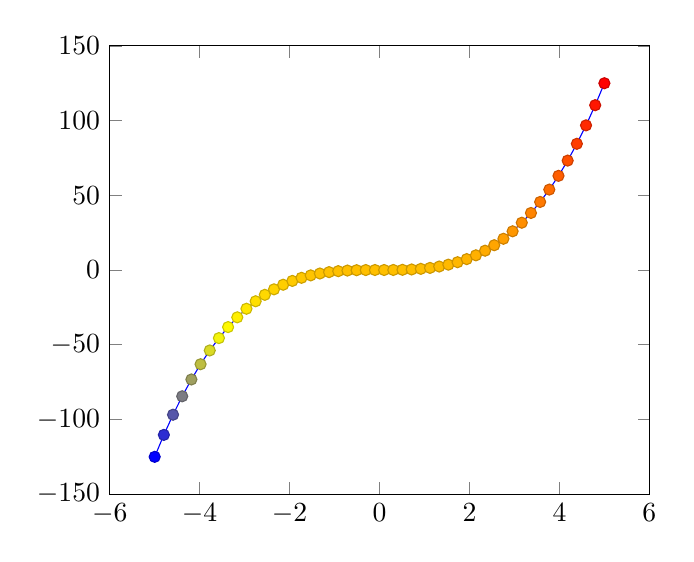
\begin{tikzpicture}
	\begin{axis}
        	\addplot+[scatter,
        		 samples=50,scatter src=y]
        		  {x^3};
        	\end{axis}
        \end{tikzpicture}
      \end{flushright}
    \end{column}
  \end{columns}
\end{frame}

\begin{frame}
  \frametitle{\TeX---\LaTeX\  Stack Excange}

  \small
  Een vraag-en-antwoordforum voor alle \LaTeX-gerelateerde zaken:
  \begin{enumerate}
    \item 60000+ vragen over \LaTeX, \url{http://tex.stackexchange.com/questions?sort=votes} is een goede manier om snel veel over \LaTeX\ te leren
    \item 7000+ vragen over \TikZ, voor een overzicht zie \url{http://tex.stackexchange.com/questions/tagged/tikz-pgf}
  \end{enumerate}
\end{frame}


\begin{frame}{Example Neural Networks}
    % \resizebox{!}{0.6\textheight}{%
    %     
% NEURAL NETWORK activation
% https://www.youtube.com/watch?v=aircAruvnKk&list=PLZHQObOWTQDNU6R1_67000Dx_ZCJB-3pi&index=1
\begin{tikzpicture}[x=2.7cm,y=1.6cm]
  \message{^^JNeural network activation}
  \def\NI{5} % number of nodes in input layers
  \def\NO{4} % number of nodes in output layers
  \def\yshift{0.4} % shift last node for dots
  
  % INPUT LAYER
  \foreach \i [evaluate={\c=int(\i==\NI); \y=\NI/2-\i-\c*\yshift; \index=(\i<\NI?int(\i):"n");}]
              in {1,...,\NI}{ % loop over nodes
    \node[node in,outer sep=0.6] (NI-\i) at (0,\y) {$a_{\index}^{(0)}$};
  }
  
  % OUTPUT LAYER
  \foreach \i [evaluate={\c=int(\i==\NO); \y=\NO/2-\i-\c*\yshift; \index=(\i<\NO?int(\i):"m");}]
    in {\NO,...,1}{ % loop over nodes
    \ifnum\i=1 % high-lighted node
      \node[node hidden]
        (NO-\i) at (1,\y) {$a_{\index}^{(1)}$};
      \foreach \j [evaluate={\index=(\j<\NI?int(\j):"n");}] in {1,...,\NI}{ % loop over nodes in previous layer
        \draw[connect,white,line width=1.2] (NI-\j) -- (NO-\i);
        \draw[connect] (NI-\j) -- (NO-\i)
          node[pos=0.50] {\contour{white}{$w_{1,\index}$}};
      }
    \else % other light-colored nodes
      \node[node,blue!20!black!80,draw=myblue!20,fill=myblue!5]
        (NO-\i) at (1,\y) {$a_{\index}^{(1)}$};
      \foreach \j in {1,...,\NI}{ % loop over nodes in previous layer
        %\draw[connect,white,line width=1.2] (NI-\j) -- (NO-\i);
        \draw[connect,myblue!20] (NI-\j) -- (NO-\i);
      }
    \fi
  }
  
  % DOTS
  \path (NI-\NI) --++ (0,1+\yshift) node[midway,scale=1.2] {$\vdots$};
  \path (NO-\NO) --++ (0,1+\yshift) node[midway,scale=1.2] {$\vdots$};
  
  % EQUATIONS
  \def\agr#1{{\color{mydarkgreen}a_{#1}^{(0)}}} % green a_i^j
  \node[below=16,right=11,mydarkblue,scale=0.95] at (NO-1)
    {$\begin{aligned} %\underset{\text{bias}}{b_1}
       &= \color{mydarkred}\sigma\left( \color{black}
            w_{1,1}\agr{1} + w_{1,2}\agr{2} + \ldots + w_{1,n}\agr{n} + b_1^{(0)}
          \color{mydarkred}\right)\\
       &= \color{mydarkred}\sigma\left( \color{black}
            \sum_{i=1}^{n} w_{1,i}\agr{i} + b_1^{(0)}
           \color{mydarkred}\right)
     \end{aligned}$};
  \node[right,scale=0.9] at (1.3,-1.3)
    {$\begin{aligned}
      {\color{mydarkblue}
      \begin{pmatrix}
        a_{1}^{(1)} \\[0.3em]
        a_{2}^{(1)} \\
        \vdots \\
        a_{m}^{(1)}
      \end{pmatrix}}
      &=
      \color{mydarkred}\sigma\left[ \color{black}
      \begin{pmatrix}
        w_{1,1} & w_{1,2} & \ldots & w_{1,n} \\
        w_{2,1} & w_{2,2} & \ldots & w_{2,n} \\
        \vdots  & \vdots  & \ddots & \vdots  \\
        w_{m,1} & w_{m,2} & \ldots & w_{m,n}
      \end{pmatrix}
      {\color{mydarkgreen}
      \begin{pmatrix}
        a_{1}^{(0)} \\[0.3em]
        a_{2}^{(0)} \\
        \vdots \\
        a_{n}^{(0)}
      \end{pmatrix}}
      +
      \begin{pmatrix}
        b_{1}^{(0)} \\[0.3em]
        b_{2}^{(0)} \\
        \vdots \\
        b_{m}^{(0)}
      \end{pmatrix}
      \color{mydarkred}\right]\\[0.5em]
      {\color{mydarkblue}\mathbf{a}^{(1)}} % vector (bold)
      &= \color{mydarkred}\sigma\left( \color{black}
           \mathbf{W}^{(0)} {\color{mydarkgreen}\mathbf{a}^{(0)}}+\mathbf{b}^{(0)}
         \color{mydarkred}\right)
    \end{aligned}$};
  
\end{tikzpicture}
    % }
\end{frame}



\subsubsection{Tikz by example - PGFplots}

\begin{frame}
  \frametitle{Plotting CSV files}
  \begin{columns}
      \begin{column}{.4\textwidth}
        \inputminted[lastline = 10]{latex}{tikz/pgfplots/data.dat}
    \end{column}
    \begin{column}{.6\textwidth}
      \begin{flushright}
         \begin{tikzpicture}
          \begin{axis}[
            grid=major,
            xlabel=$x$,
            ylabel=$y$
          ]
            \addplot table[x = x, y = f]
              {tikz/pgfplots/data.dat};
            \addlegendentry{$f = x^2-x+4$};
            \addplot table[x = x, y = g]
              {tikz/pgfplots/data.dat};
            \addlegendentry{$g = 0.5x^2-3x+3$};
          \end{axis}
        \end{tikzpicture}
      \end{flushright}
    \end{column}
  \end{columns}
\end{frame}


\begin{frame}
  \frametitle{Integratie met externe tools}

  \begin{description}
    \item[\texttt{matlab2tikz}] \url{https://github.com/nschloe/matlab2tikz}
      exporteer Matlab-figuren meteen naar \TikZ
    \pause
    \item[\texttt{matplotlib2tikz}] \url{https://github.com/nschloe/matplotlib2tikz}
      exporteer matplotlib-figuren meteen naar \TikZ
  \end{description}
\end{frame}


\subsubsection{Tikz Externalize in Overleaf}

% NOTE: For TikZ externalization to work on Overleaf the \tikzexternalize command must be given in the project’s main .tex file

% \tikzsetnextfilename{#1}


% The option prefix=tikz/ provides the name of a folder (here, tikz) to be used for caching generated (externalized) figures—you will need to create that folder manually in your project. However, before LaTeX (TikZ code) can write to that folder, it needs to contain a file—any (dummy) file will suffice; for example, you can add an empty text file foo.txt in the tikz folder.

\begin{frame}{}
    \ZeigerdiagrammText{60}{-90}{2.7}{1.8}
\end{frame}